\documentclass[a4paper]{article}
\usepackage{geometry}
\usepackage{graphicx}
\usepackage{natbib}
\usepackage{amsmath}
\usepackage{amssymb}
\usepackage{amsthm}
\usepackage{paralist}
\usepackage{epstopdf}
\usepackage{tabularx}
\usepackage{longtable}
\usepackage{multirow}
\usepackage{multicol}
\usepackage[hidelinks]{hyperref}
\usepackage{fancyvrb}
\usepackage{algorithm}
\usepackage{algorithmic}
\usepackage{float}
\usepackage{paralist}
\usepackage[svgname]{xcolor}
\usepackage{enumerate}
\usepackage{array}
\usepackage{times}
\usepackage{url}
\usepackage{fancyhdr}
\usepackage{comment}
\usepackage{environ}
\usepackage{times}
\usepackage{textcomp}
\usepackage{caption}
\usepackage{multirow}
\usepackage{bbm}

% \usepackage{kky}

\newcounter{thm}
\ifx\fact\undefined
\newtheorem{fact}[thm]{Fact}
\fi

\newcommand{\pen}{{\rm pen}}
\newcommand{\diag}{{\rm diag}}
\newcommand{\diam}{{\bf{\rm diam}}}
\newcommand{\spann}{{\bf{\rm span}}}
\newcommand{\nulll}{{\bf{\rm null}}}
% Distributions
\newcommand{\Bern}{{\bf{\rm Bern}}\,} % support of a function
\newcommand{\Categ}{{\bf{\rm Categ}}\,} % support of a function
\newcommand{\Mult}{{\bf{\rm Mult}}\,} % support of a function
\newcommand{\Dir}{{\bf{\rm Dir}}\,} % support of a function
\newcommand{\horizontalline}{\noindent\rule[0.5ex]{\linewidth}{1pt}}
\newcommand{\HRule}{\rule{\linewidth}{0.5mm}} 
\newcommand{\Hrule}{\rule{\linewidth}{0.3mm}}
\newcommand{\HRuleN}{\HRule\\} 
\newcommand{\HruleN}{\Hrule\\}
\newcommand{\superscript}[1]{{\scriptsize \ensuremath{^{\textrm{#1}}}}}
\newcommand{\supindex}[2]{#1^{(#2)}}
\newcommand{\xii}[1]{\supindex{x}{#1}}
\newcommand{\yii}[1]{\supindex{y}{#1}}
\newcommand{\zii}[1]{\supindex{z}{#1}}
\newcommand{\Xii}[1]{\supindex{X}{#1}}
\newcommand{\Yii}[1]{\supindex{Y}{#1}}
\newcommand{\Zii}[1]{\supindex{Z}{#1}}
\newcommand{\NN}{\mathbb{N}} % Natural numbers
\newcommand{\Ncal}{\mathcal{N}}
\newcommand{\Dcal}{\mathcal{D}}
\newcommand{\Lcal}{\mathcal{L}}
\newcommand{\Xcal}{\mathcal{X}}
\newcommand{\Pcal}{\mathcal{P}}
\newcommand{\Jcal}{\mathcal{J}}
\newcommand{\Rcal}{\mathcal{R}}
\newcommand{\indfone}{\mathbbm{1}}
\newcommand{\gb}{\mathbf{g}}
\newcommand{\Hb}{\mathbf{H}}
\newcommand{\Db}{\mathbf{D}}
\newcommand*{\zero}{{\bf 0}}
\newcommand*{\one}{{\bf 1}}

% Stuff mostly appearing in Statistics
\newcommand{\Xbar}{\bar{X}}
\newcommand{\Ybar}{\bar{Y}}
\newcommand{\Zbar}{\bar{Z}}
\newcommand{\Xb}{\mathbf{X}}


%%%%  brackets
\newcommand{\inner}[2]{\left\langle #1,#2 \right\rangle}
\newcommand{\rbr}[1]{\left(#1\right)}
\newcommand{\sbr}[1]{\left[#1\right]}
\newcommand{\cbr}[1]{\left\{#1\right\}}
\newcommand{\nbr}[1]{\left\|#1\right\|}
\newcommand{\abr}[1]{\left|#1\right|}

% derivatives and partial fractions
\newcommand{\differentiate}[2]{ \frac{ \ud #2}{\ud #1} }
\newcommand{\differentiateat}[3]{ \frac{ \ud #2}{\ud #1}  \Big|_{#1=#3} }
\newcommand{\partialfrac}[2]{ \frac{ \partial #2}{\partial #1} }
\newcommand{\partialfracat}[3]{ \frac{ \partial #2}{\partial #1} \Big|_{#1=#3} }
\newcommand{\partialfracorder}[3]{ \frac{ \partial^{#3} #2}{\partial^{#3} #1} }
\newcommand{\partialfracatorder}[4]{ \frac{ \partial^{#3} #2}{\partial^{#3} #1} \Big|_{#1=#4} }

\urlstyle{rm}

\setlength\parindent{0pt} % Removes all indentation from paragraphs
\theoremstyle{definition}
\newtheorem{definition}{Definition}[]
\newtheorem{conjecture}{Conjecture}[]
\newtheorem{example}{Example}[]
\newtheorem{theorem}{Theorem}[]
\newtheorem{lemma}{Lemma}
\newtheorem{proposition}{Proposition}
\newtheorem{corollary}{Corollary}


\floatname{algorithm}{Procedure}
\renewcommand{\algorithmicrequire}{\textbf{Input:}}
\renewcommand{\algorithmicensure}{\textbf{Output:}}
\newcommand{\abs}[1]{\lvert#1\rvert}
\newcommand{\norm}[1]{\lVert#1\rVert}
\newcommand{\RR}{\mathbb{R}}
\newcommand{\EE}{\mathbb{E}}
\newcommand{\PP}{\mathbb{P}}
\newcommand{\CC}{\mathbb{C}}
\newcommand{\Nat}{\mathbb{N}}
\newcommand{\br}[1]{\{#1\}}
\DeclareMathOperator*{\argmin}{arg\,min}
\DeclareMathOperator*{\argmax}{arg\,max}
\renewcommand{\qedsymbol}{$\blacksquare$}

\definecolor{dkgreen}{rgb}{0,0.6,0}
\definecolor{gray}{rgb}{0.5,0.5,0.5}
\definecolor{mauve}{rgb}{0.58,0,0.82}

\newcommand{\Var}{\mathrm{Var}}
\newcommand{\Cov}{\mathrm{Cov}}

\newcommand{\vc}[1]{\boldsymbol{#1}}
\newcommand{\xv}{\vc{x}}
\newcommand{\Sigmav}{\vc{\Sigma}}
\newcommand{\alphav}{\vc{\alpha}}
\newcommand{\muv}{\vc{\mu}}

\newcommand{\red}[1]{\textcolor{red}{#1}}

\def\x{\mathbf x}
\def\y{\mathbf y}
\def\w{\mathbf w}
\def\v{\mathbf v}
\def\E{\mathbb E}
\def\V{\mathbb V}

% TO SHOW SOLUTIONS, include following (else comment out):
\newenvironment{soln}{
    \leavevmode\color{blue}\ignorespaces
}{}

\hypersetup{
%    colorlinks,
    linkcolor={red!50!black},
    citecolor={blue!50!black},
    urlcolor={blue!80!black}
}

\geometry{
  top=1in,            % <-- you want to adjust this
  inner=1in,
  outer=1in,
  bottom=1in,
  headheight=3em,       % <-- and this
  headsep=2em,          % <-- and this
  footskip=3em,
}


\pagestyle{fancyplain}
\lhead{\fancyplain{}{Homework 5}}
\rhead{\fancyplain{}{CS 760 Machine Learning}}
\cfoot{\thepage}

\title{\textsc{Homework 5}} % Title

%%% NOTE:  Replace 'NAME HERE' etc., and delete any "\red{}" wrappers (so it won't show up as red)

\author{
\red{$>>$NAME HERE$<<$} \\
\red{$>>$ID HERE$<<$}\\
}

\date{}

\begin{document}

\maketitle 


\textbf{Instructions:}
Use this latex file as a template to develop your homework. We are changing our reproducibility policy on code submissions going forward. \textbf{Instead of uploading it on GitHub, please submit a separate zip file that contains your code. You will submit two files to Canvas, one is your pdf, and the other one is a zip file.} Late submissions may not be accepted. You can choose any programming language (i.e. python, R, or MATLAB). Please check Piazza for updates about the homework.
\vspace{0.1in}

This homework is more difficult than previous homework. The total amount of points for this homework is \textbf{150}. The extra credit reflects the level of difficulty.

\vspace{0.1in}

\section{Clustering}

\subsection{K-means Clustering (14 points)}

\begin{enumerate}

\item \textbf{(6 Points)}
Given $n$ observations $X_1^n = \{X_1, \dots, X_n\}$, $X_i \in \Xcal$, the K-means objective
is to find $k$
($<n$) centres $\mu_1^k = \{\mu_1, \dots, \mu_k\}$, and a rule $f:\Xcal \rightarrow
\{1,\dots, K\}$ so as to minimize the objective

\begin{equation}
J(\mu_1^K, f; X_1^n) = \sum_{i=1}^n \sum_{k=1}^K \indfone(f(X_i) = k) \|X_i - \mu_k\|^2
\label{eqn:kmeans}
\end{equation}

Let $\Jcal_K(X_1^n) = \min_{\mu_1^k, f} J(\mu_1^K, f; X_1^n)$. Prove that
$\Jcal_{K}(X_1^n)$ is a non-increasing function of $K$.

\begin{soln}
Lets begin by finding what $f,\mu_K$ are. Although we cannot find the best $\mu$ and $f$ at the same time, we can:
\begin{itemize}
    \item fix $\mu$, we find the best $f$ exactly. Also called the Assignment Step.
    \begin{align*}
        \Jcal_K(X_1^n) &= \min_{f} J(\mu_1^K, f; X_1^n)\\
        &= \min_{f} \sum_{i=1}^n \sum_{k=1}^K \indfone(f(X_i) = k) \|X_i - \mu_k\|^2 \\
        &= \min_{f} \sum_{k=1}^K \indfone(f(X_1) = k) \|X_1 - \mu_k\|^2 + \ldots + \sum_{k=1}^K \indfone(f(X_n) = k) \|X_n - \mu_k\|^2
    \end{align*}
    Thus we can minimize each of the above term individually by setting
    $$
        f(X_i) = \argmin_{k} \|X_i - \mu_k\|^2
    $$
    \textbf{Which means to assign the point to the cluster whose centroid is closest.}
    \item fix $f$, we find the best $\mu$ exactly. Also called the Update Step.
    \begin{align*}
        \Jcal_K(X_1^n) &= \min_{\mu_1^K} J(\mu_1^K, f; X_1^n)\\
        &= \min_{\mu_1^K} \sum_{i=1}^n \sum_{k=1}^K \indfone(f(X_i) = k) \|X_i - \mu_k\|^2 \\
        &= \min_{\mu_1^K} \sum_{i=1}^n \indfone(f(X_i) = 1) \|X_i - \mu_1\|^2 + \ldots + \sum_{i=1}^n \indfone(f(X_i) = K) \|X_i - \mu_K\|^2
    \end{align*}
    The individual terms can be minimized by setting:
    $$
        \mu_k = \argmin_{\mu} \sum_{i=1}^n\indfone(f(X_i) = k)\|X_i - \mu\|^2 = \frac{\sum_{i=1}^n\indfone(f(X_i) = k)X_i}{\sum_{i=1}^n\indfone(f(X_i) = k)}
    $$
    \textbf{Thus pick a centroid of a cluster as the mean of all points in that cluster.}
\end{itemize}

Now lets pick a setting where we increase the number of clusters by 1 i.e. total clusters are $\mathbf{K+1}$. \\
Let $f^{K}(X_i)$ assign the cluster to a point in a setting with K cliusters.
    
\begin{itemize}
    \item Assignment Step proof: 
    
    A point will be assigned to this new cluster if and only if its closer to the center of this new cluster
    $$
        \|X_i - \mu_{K+1}\|^2 < \|X_i - \mu_{k}\|^2 \;\forall\;k=1,2,...,K
    $$ 
    Thus decreasing the total objective value than before. The worst case scenario is when no point is assigned to this new cluster in which case the objective value remains the same.\\
    
    \textbf{Hence proved the objective value can never increase during assignment step when increasing $K$.}

    \item Update Step proof:
    If a point is assigned from cluster $k$ to $K+1$. 
    \begin{itemize}
        \item Let the cluster $k$ with less points be called $k'$. \\
        The new $\mu_{k'}$ will change from before if and only if it decreases the total objective value of leftover points in its cluster. If the new $\mu_{k'}$ increases the total objective value then it was better off staying at $\mu_k$.
        $$
            \sum_{i=1}^n\indfone(f^{K+1}(X_i) = k')\|X_i - \mu_{k'}\|^2 \leq \sum_{i=1}^n\indfone(f^{K+1}(X_i) = k')\|X_i - \mu_{k}\|^2
        $$
        \item As for the point assigned to $K+1$.\\
        % We can easily say $\|X_i - \mu_{k}\|^2 \leq \|X_i - \mu_{k'}\|^2$, otherwise $\mu_{k'}$ would have been the original centroid for cluster $k$ as it reduces the distance of all points in the original cluster.\\
        Now if the sum of objective value in the original setting is less than in the current one i.e.:
        $$
            \sum_{i=1}^n\indfone(f^{K+1}(X_i) = K+1)\|X_i - \mu_{f^{K}(X_i)}\|^2 \leq \sum_{i=1}^n\indfone(f^{K+1}(X_i) = K+1)\|X_i - \mu_{K+1}\|^2
        $$
        Where $\mu_{f^{K}(X_i)}$ is the centroid of their cluster in the original setting with only K cluster \\
        Then:
        $$
            \mu = \frac{\sum_{i=1}^n\indfone(f^{K+1}(X_i) = K+1)\mu_{f^{K}(X_i)}}{\sum_{i=1}^n\indfone(f^{K+1}(X_i) = K+1)}
        $$
        gives equal objective value as the original setting and is a better choice of $\mu_{K+1}$. Thus the sum of objective values for newly assigned points can also never increase.
    \end{itemize}
    \textbf{Thus increasing $K$ will increase the total objective value for neither the set of points that don't change cluster nor those which do during the Update Step.}
\end{itemize}
\end{soln}

\item \textbf{(8 Points)}
Consider the K-means (Lloyd's) clustering algorithm we studied in class. We
terminate the algorithm when there are no changes to the objective.
Show that the algorithm terminates in a finite number of steps.

\begin{soln}
    We can see above that the K-mean algorithm moves in a fashion to reduce the objective $\Jcal_K(X_1^n) = \min_{\mu_1^k, f} J(\mu_1^K, f; X_1^n)$. Now for \textbf{fixed set of points} $X_1^n = \{X_1, \dots, X_n\}$, $X_i \in \Xcal$ and a \textbf{fixed $K$} there can only be a finite set of assignments of points to the clusters i.e. only a \textbf{finite number of objective values} and even if the algorithm iterates over all of them it will eventually choose the one with minimum objective value $\Jcal_K(X_1^n)$ and terminate after those finite set of iterations and converge to a solution. 
\end{soln}

\end{enumerate}



\subsection{Experiment (20 Points)}

In this question, we will evaluate
K-means clustering and GMM on a simple 2 dimensional problem.
First, create a two-dimensional synthetic dataset of 300 points by sampling 100 points each from the
three Gaussian distributions shown below:
\[
P_a = \Ncal\left(
\begin{bmatrix}
-1 \\ -1
\end{bmatrix},
\;
\sigma\begin{bmatrix}
2, &0.5 \\ 0.5, &1
\end{bmatrix}
\right),
\quad
P_b = \Ncal\left(
\begin{bmatrix}
1 \\ -1
\end{bmatrix},
\;
 \sigma\begin{bmatrix}
1, &-0.5 \\ -0.5, &2
\end{bmatrix}
\right),
\quad
P_c = \Ncal\left(
\begin{bmatrix}
0 \\ 1
\end{bmatrix},
\;
 \sigma\begin{bmatrix}
1 &0 \\ 0, &2
\end{bmatrix}
\right)
\]
Here, $\sigma$ is a parameter we will change to produce different datasets.

\begin{soln}
    \begin{figure}[H]
        \begin{subfigure}{0.5\textwidth}
            \centering
            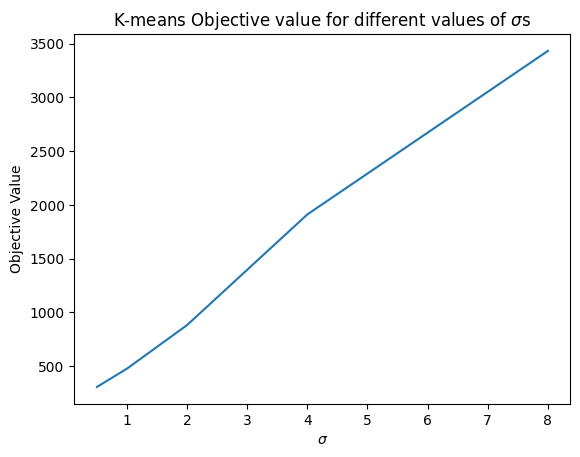
\includegraphics[scale=0.35]{Images/q12/q12_km.png}
        \end{subfigure}%
        \begin{subfigure}{0.5\textwidth}
            \centering
            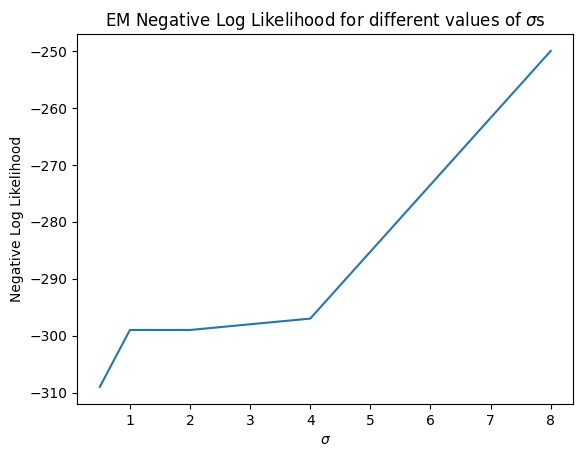
\includegraphics[scale=0.35]{Images/q12/q12_em.png}
        \end{subfigure}
    \end{figure}
    \begin{figure}[H]
        \centering
        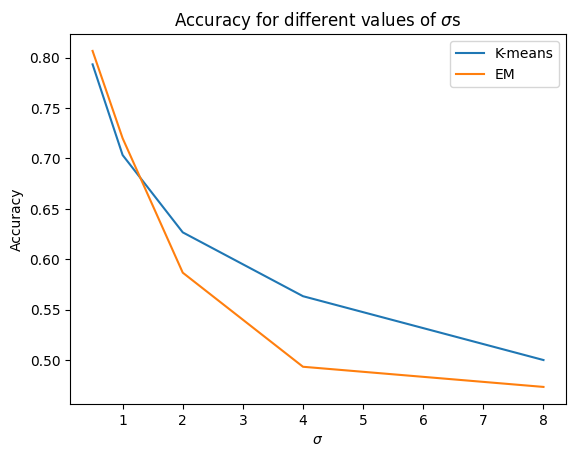
\includegraphics[scale=0.4]{Images/q12/q12_acc.png}
    \end{figure}
\end{soln}

\begin{itemize}
\item First implement K-means clustering and the expectation maximization algorithm for GMMs.
Execute both methods on five synthetic datasets,
generated as shown above with $\sigma \in \{0.5, 1, 2, 4, 8\}$. Finally, evaluate both methods on \emph{(i)} the clustering objective~\eqref{eqn:kmeans} and \emph{(ii)}  the clustering accuracy. For each of the two criteria, plot the value achieved by each method against $\sigma$.

\item Both algorithms are only guaranteed to find only a local optimum so we recommend trying multiple
restarts and picking the one with the lowest objective value (This is~\eqref{eqn:kmeans} for K-means and the negative log likelihood for GMMs).
You may also experiment with a smart initialization
strategy (such as kmeans++).

\item
To plot the clustering accuracy,  you may treat the `label' of points generated from distribution
$P_u$ as $u$, where $u\in \{a, b, c\}$.
Assume that the cluster id $i$ returned by a method is $i\in \{1, 2, 3\}$.
Since clustering is an unsupervised learning problem, you should obtain the best possible mapping
from $\{1, 2, 3\}$ to $\{a, b, c\}$ to compute the clustering objective.
One way to do this is to compare the clustering centers returned by the method (centroids for
K-means, means for GMMs) and map them to the distribution with the closest mean.

\end{itemize}

Points break down: 7 points each for implementation of each method, 6 points for reporting of
evaluation metrics.

\section{Linear Dimensionality Reduction}

\subsection{Principal Components Analysis  (10 points)}
\label{sec:pca}

Principal Components Analysis (PCA) is a popular method for linear dimensionality reduction. PCA attempts to find a lower dimensional subspace such that when you project the data onto the subspace as much of the information is preserved. Say we have data $X = [x_1^\top; \dots; x_n^\top] \in \RR^{n\times D}$ where  $x_i \in \RR^D$. We wish to find a $d$ ($ < D$) dimensional subspace $A = [a_1, \dots, a_d] \in \RR^{D\times d}$, such that $ a_i \in \RR^D$ and $A^\top A = I_d$, so as to maximize $\frac{1}{n} \sum_{i=1}^n \|A^\top x_i\|^2$.
\begin{enumerate}

\item  \textbf{(4 Points)}
Suppose we wish to find the first direction $a_1$ (such that $a_1^\top a_1 = 1$) to maximize $\frac{1}{n} \sum_i (a_1^\top x_i)^2$.
Show that $a_1$ is the first right singular vector of $X$.

\begin{soln}
    We have $a_1^\top x_i = x_i^\top a_1$
    $$
    \max_{||a||^2_2=1}\frac{1}{n}\sum_i(a_1^\top x_i)^2 = \max_{||a||^2_2=1}\frac{1}{n}\sum_i(a_1^\top x_i)(x_i^\top a_1) = \max\frac{1}{n}\sum_i(a_1^\top x_ix_i^\top a_1)
    $$
    Now for the above expression
    $$
        \frac{1}{n}\sum_ix_ix_i^\top=\frac{1}{n}X^\top X \\
    $$
    From the Singular Value Decomposition of X
    \begin{align*}
        X &= U \Sigma V^\top \\
        X^\top X &= V\Sigma^\top U^\top U\Sigma V^\top \\
        &= V\Sigma^\top\Sigma V^T 
    \end{align*}
    
    Follows from the fact that $U^TU =I$ \\
    Substituting above:\\
    $$
        \max\frac{1}{n} a_1^T X^T X a_1 = \max\frac{1}{n} a_1^T V \Sigma^2 V^T a_1
    $$
    Let $z=V^T a_1$ :  
    $$
        \max\frac{1}{n} z^T \Sigma^2 z = \max\frac{1}{n}\text{tr}(z^T \Sigma^2 z) =  \max\frac{1}{n}\text{tr}(zz^T \Sigma^2) = max\frac{1}{n} \sum_{i=1}^D \sigma_i^2z_i^2
    $$
    Now if $V = [v_1, \dots, v_D] \in \RR^{D\times D}$, such that $v_i \in \RR^D$. Each element of $Z$ is $z_i = v_i^\top a_1$ is the projection of $a_1$ on the orthogonal set of vectors of $V$. Now we know $\sigma_1^2 > \sigma_2^2 > \dots > \sigma_D^2$. 
    
    Thus to maximize the objective function the factor of $\sigma_1$ needs to be the largest i.e. $\mathbf{v_1^\top a_1 > v_i^\top a_1}\;\forall i\neq 1$. Knowing that $v_i$ are a set of orthogonal vectors the mentioned criteria can only be achieved if $\mathbf{v_1=a_1}$. Hence Proved
    
\end{soln}

\item  \textbf{(6 Points)}
Given $a_1, \dots, a_k$, let $A_k = [a_1, \dots, a_k]$ and 
$\tilde{x}_i = x_i - A A^\top x_i$. We wish to find $a_{k+1}$, to maximize
$\frac{1}{n} \sum_i (a_{k+1}^\top \tilde{x}_i)^2$. Show that $a_{k+1}$ is the
$(k+1)^{th}$ right singular vector of $X$.

\begin{soln}
    \begin{gather*}
        \tilde{x}_i = x_i - A A^\top x_i \\
        (x_i^\top AA^\top) \cdot \tilde{x}_i = (x_i^\top AA^\top) \cdot (x_i - A A^\top x_i) = (x_i^\top AA^\top x_i) - (x_i^\top AA^\top x_i) = 0
    \end{gather*} 
    Therefore $x_i^\top AA^\top \perp x_i - A A^\top x_i$ \\
    Now,
    $$
    A A^\top x_i = \sum_{j=1}^{k} a_ja_j^\top x_i = \sum_{j=1}^{k} a_jx_i^\top a_j = \sum_{j=1}^{k} (x_i^\top a_j)a_j = x_i^\top AA^\top \Rightarrow A A^\top x_i \perp x_i - A A^\top x_i
    $$
    Consequently $\|x_i\|^2 = \|A A^\top x_i\|^2 + \|x_i - A A^\top x_i\|^2$ \\
    Thus $\tilde{x}_i$ is the component of $x_i$ orthogonal to $AA^\top x_i$ and is a way to split $x_i$ into two orthogonal components.\\
    Stacking $x_i^\top$ we get $\tilde{X}^\top = X^\top - AA^\top X^\top$
    $$
        AA^\top X^\top = XAA^\top = U \Sigma V^\top A A^\top
    $$
    From the previous proof we can see every row of $V^\top A$ is $v_iA$ which is a $(1\times k)$ row vector with 1 at $i^{th}$ place and 0 at all other places up-to the $k_{th}$ vector and a zero for all vectors from $k+1$ to $D$. This gives us,
    $$
        U \Sigma V^\top A A^\top = \sum_i^D \sigma_i u_i v_i^T A A^T = \sum_i^k \sigma_i u_i v_i
    $$
    Thus $\tilde{X}$ is essentially equal to removing the approximation of X along the first k components of right singular vector from $X$ or removing the best-k-rank approximation of $X$ from itself. Hence our problem boils down to 
    $$
        \max \frac{1}{n} \sum_i (a_{k+1}^\top \tilde{x}_i)^2 = \max\frac{1}{n} \sum_{k+1}^D \sigma_i^2z_i^2
    $$
    Where $z_i = v_i^\top a_{k+1}$ and following from the proof in 2.1.1 this is maximized when $\mathbf{a_{k+1}=v_{k+1}}$
\end{soln}



% \item \textbf{(2 Points)}
% You are given a point $z_*$ in the $d$ dimensional space obtained using PCA.
% What is $x_*$, the reconstruction of $z_*$ in the original $D$ dimensional space?



\end{enumerate}


\subsection{Dimensionality reduction via optimization (22 points)}

We will now motivate the dimensionality reduction problem from a slightly different
perspective. The resulting algorithm has many similarities to PCA.
We will refer to method as DRO.

As before, you are given data $\{x_i\}_{i=1}^n$, where $x_i \in \RR^D$. Let $X=[x_1^\top; \dots
x_n^\top] \in \RR^{n\times D}$. We suspect that the data
actually lies approximately in  a $d$ dimensional affine subspace.
Here $d<D$ and $d<n$.
Our goal, as in PCA, is to use this dataset to find a $d$ dimensional representation $z$ for each $x\in\RR^D$.
(We will assume that the span of the data has dimension larger than
$d$, but our method should work whether $n>D$ or $n<D$.)


Let $z_i\in \RR^d$ be the lower dimensional representation for $x_i$ and
let $Z = [z_1^\top; \dots; z_n^\top] \in \RR^{n\times d}$.
We wish to find parameters $A \in \RR^{D\times d}$, $b\in\RR^D$ and the lower
dimensional representation $Z\in \RR^{n\times d}$ so as to minimize 
\begin{equation}
J(A,b,Z) = \frac{1}{n} \sum_{i=1}^n \|x_i - Az_i - b\|^2 = \| X - ZA^\top - \one b^\top\|_F^2.
\label{eqn:dimobj}
\end{equation}
Here, $\|A\|^2_F = \sum_{i,j} A_{ij}^2$ is the Frobenius norm of a matrix.


\begin{enumerate}
\item \textbf{(3 Points)}
Let $M\in\RR^{d\times d}$ be an arbitrary invertible matrix and $p\in\RR^{d}$ be an arbitrary vector.
Denote, $A_2 = A_1M^{-1}$, $b_2 = b_1- A_1M^{-1}p$ and $Z_2 = Z_1 M^\top +
\one p^\top$.
Show that both
$(A_1, b_1, Z_1)$ and $(A_2, b_2, Z_2)$ achieve the same objective value $J$~\eqref{eqn:dimobj}.
\end{enumerate}

\begin{soln}
    \begin{gather*}
        J(A_1,b_1,Z_1) = \| X - Z_1A_1^\top - \one b_1^\top\|_F^2.
    \end{gather*}
    \begin{gather*}
        J(A_2,b_2,Z_2) = \| X - Z_2A_2^\top - \one b_2^\top\|_F^2.
    \end{gather*}
    Substituting the given values\\
    $A_2 = A_1M^{-1}$, $b_2 = b_1- A_1M^{-1}p$ and $Z_2 = Z_1 M^\top + \one p^\top$. \\
    \begin{gather*}
        J(A_2,b_2,Z_2) = \| X - (Z_1 M^\top + \one p^\top)(A_1M^{-1})^\top - \one (b_1 -A_1M^{-1}p)^\top\|_F^2\\       
        J(A_2,b_2,Z_2) = \| X - Z_1 M^\top (M^{-1})^\top A_1^\top - p^\top (M^{-1})^\top A_1^{\top} - b_1^\top +p^\top (M^{-1})^\top A_1^\top\|_F^2\\         
        J(A_2,b_2,Z_2) = \| X - Z_1 (M^{-1} M)^\top A_1^\top  - \one b_1^\top \|_F^2\\
        J(A_2,b_2,Z_2) = \| X - Z_1  A_1^\top - \one b_1^\top\|_F^2 = J(A_1,b_1,Z_1)\\
    \end{gather*}
Hence, we can observe above that both objectives are equal.
\end{soln}

Therefore, in order to make the problem determined, we need to impose some
constraint on $Z$. We will assume that the $z_i$'s have zero mean and identity covariance.
That is,
\begin{align*}
\Zbar = \frac{1}{n} \sum_{i=1}^n z_i =\frac{1}{n} Z^\top {\bf 1}_n = 0, \hspace{0.3in} 
S = \frac{1}{n} \sum_{i=1}^n z_i z_i^\top 
= \frac{1}{n} Z^\top Z
= I_d
\end{align*}
Here, ${\bf 1}_d = [1, 1 \dots, 1]^\top \in\RR^d$ and $I_d$  is the $d\times d$ identity matrix.

\begin{enumerate}
\setcounter{enumi}{1}
\item \textbf{(16 Points)}
Outline a procedure to solve the above problem. Specify how you
would obtain $A, Z, b$ which minimize the objective and satisfy the constraints.

\textbf{Hint: }The rank $k$ approximation of a matrix in Frobenius norm is obtained by
taking its SVD and then zeroing out all but the first $k$ singular values.

\begin{soln}\\
    We need to minimize:
    $$
        g(x_i,z_i|A,b) = \frac{1}{n} \sum_{i=1}^n \|x_i - Az_i - b\|^2 = \| X - ZA^\top - \one b^\top\|_F^2
    $$
    
    What we are trying to achieve here is express $X$ in a lower dimensional basis of $Z$ and then reduce the reconstruction error when reverting from $z$-space back to $x$-space.
    
    Lets assume our new basis space as $A = [a_1;a_2;\dots;a_d]$ such that $a_i \in \RR^D$ and $a_i \perp a_j \;\forall\;i\neq j$ and $b$ is added to account for any shift in centre of $X$.

    Coordinate in lower dimension $d$: 
    $$
        z^i_j=(x_i-b)^\top a_j\;\forall\;i\in[1,n];j\in[1,d]
    $$

    First lets solve for b:
    \begin{gather*}
        \nabla_b g(x_i,z_i|A,b) = \frac{2}{n}\sum_{i=1}^{n}(x_i - Az_i -b) = 0 \\
        \Rightarrow \sum_{i=1}^{n}x_i - A\sum_{i=1}^{n}z_i - nb = 0 \\
        \Rightarrow \sum_{i=1}^{n}x_i - 0 - nb = 0 \\
        \Rightarrow \mathbf{b = \frac{1}{n}\sum_{i=1}^{n}x_i}
    \end{gather*}
    
    Now we need to find $A = [a_1;a_2;\dots;a_d]$ by minimizing:
    $$
        \frac{1}{n} \sum_{i=1}^n \|x_i - b-\sum_{j=1}^dz^i_ja_j\|^2
    $$
    Now we should also note that $x_i$ can be represented by a n-dimensional projection as $x_i=b+\sum_{j=1}^n a_j z^i_j$:\\
    Substituting :
    \begin{gather*}
        \frac{1}{n} \sum_{i=1}^n \| (b+\sum_{j=1}^n a_j z^i_j)- (b+\sum_{j=1}^d a_j z^i_j)\|^2 = \frac{1}{n} \sum_{i=1}^n \| (\sum_{j=d+1}^n a_j z^i_j )\|^2 \\
        \Rightarrow \implies  \frac{1}{n} \sum_{i=1}^n (\left(\sum_{j=d+1}^n z^{i}_j a_j^T\right) \left(\sum_{j=d+1}^n a_j z^i_j \right)) \\
        \Rightarrow  \frac{1}{n} \sum_{i=1}^n (\sum_{j=d+1}^n (z^{i}_j)^2 )
    \end{gather*}
This follows from the fact that $a_i \perp a_j \;\forall\;i\neq j$\\
Substituting value of $z_i$
$$
\frac{1}{n} \sum_{i=1}^n \sum_{j=d+1}^n(a^T_j(x_i-b)(x_i - b)^T a_j)
$$
$$\implies
 \frac{1}{n} \sum_{j=d+1}^n (a^T_j[\sum_{i=1}^n(x_i-\bar x)(x_i - \bar x)^T] a_j)
$$
This is nothing but the covariance matrix. So our optimization becomes\\
$$
\min \sum_{j=d+1}^n(a^T_j\Sigma a_j)
$$
Where $\Sigma=\frac{1}{n}\sum_{i=1}^n(x_i-\frac{1}{n}\sum_{i=1}^{n}x_i)(x_i - \frac{1}{n}\sum_{i=1}^{n}x_i)^T$\\

To minimize the above i.e, $j=d+1\to n$ is equivalent to maximizing $j=1\to d$. \textit{This follows from the fact that $a_{d+1}$ to $a_n$, need to explain the least variance in demeaned $X$, thus in turn $a_1$ to $a_d$ need to explain the maximum variance in $X$.} Arriving again at the condition where we have to :\\
$$
\max \sum_{j=1}^d(a^T_j\Sigma a_j)
$$
This can be maximized by setting $\mathbf{a_j}$'s in the direction of \textbf{right singular values of demeaned} $\mathbf{X}$ and picking the \textbf{first $\mathbf{d}$ right singular vectors} as proven already in 2.1.1.
\end{soln}

\item \textbf{(3 Points)}
You are given a point $x_*$ in the original $D$ dimensional space.
State the rule to obtain the $d$ dimensional
representation $z_*$ for this new point.
(If $x_*$ is some original point $x_i$ from the $D$--dimensional space, it shoud be the $d$--dimensional representation $z_i$.)

\begin{soln}
    $$
        z_* = (x_* - b)^\top A
    $$
\end{soln}


%\item \textbf{(1 Point)}
% You are given a point $z_*$ in the $d$ dimensional space obtained using DRO.
% What is $x_*$, the reconstruction of $z_*$ in the original $D$ dimensional space?

\end{enumerate}


\subsection{Dimensionality reduction via a generative model (42 points)}

We will now study dimensionality reduction via a generative model.
We will refer to method as DRLV.
We will assume a $d (<n)$ dimensional latent space and
the following generative process for the data.
\begin{align*}
& z \sim \Ncal(\zero, I),  \quad  z\in \RR^d \\
& x|z \sim \Ncal(Az + b, \eta^2 I),  \quad  x\in \RR^D 
\end{align*}
The model says that we first sample a $d$ dimensional Gaussian with zero mean
and identity variance. Then we map it to $D$ dimensions by computing $Az+b$.
Finally, we add some spherical Gaussian noise with variance $\eta^2$ on each
dimension.

We will use an expectation maximization (EM)
procedure to learn the parameters $A, b, \eta$. So far we have only studied
 EM with discrete latent variables. In this problem, we will look at
EM with a continuous latent variable which has a parametric distribution.
The following results will be useful.\\

\begin{fact}[Conditional of a Gaussian]
Say $(Y_1, Y_2), Y_i \in \RR^{d_i}$ is Gaussian distribued.
\[
\left(\begin{array}{c}Y_1 \\ Y_2\end{array}\right) =
\Ncal \left( \left(\begin{array}{c} \mu_1 \\ \mu_2 \end{array} \right), 
\left[ \begin{array}{cc} \Sigma_{11} & \Sigma_{12} \\ \Sigma_{12}^\top &
  \Sigma_{22} \end{array} \right] 
  \right)
\]
Then, conditioned on $Y_1 = y_1$ the distribution for $Y_2$ is
\[
Y_2 | Y_1 = y_1 \sim \Ncal(\mu_2+ \Sigma_{12}^\top \Sigma_{11}^{-1} (y_1 - \mu_1), \;
  \Sigma_{22} - \Sigma_{12}^\top \Sigma_{11}^{-1}\Sigma_{12} )
\]
\end{fact}

\begin{fact}[Some Matrix Derivatives]
Let $X\in \RR^{r\times c}$, and $u\in \RR^r$, $v,w \in \RR^c$.
\begin{align*}
\nabla_X v^\top X^\top u &= uv^\top \\
\nabla_X v^\top X^\top X w &= X(vw^\top + wv^\top)
\end{align*}
\end{fact}
\vspace{0.1in}

\begin{enumerate}
\item \textbf{(10 Points)}
Assuming some given values for $A$, $b$, and $\eta^2$, write down the joint distribution of $(z,x)$. Use this to derive the marginal
distribution of $x$ and the conditional distribution $z|x$.

\begin{soln}
    \begin{gather*}
        p(z) = \frac{1}{{(2\pi)}^{d/2}}\exp{\left(-\frac{1}{2}z^\top z\right)} \\
        p(x|z) = \frac{1}{\eta{(2\pi)}^{D/2}}\exp{\left(-\frac{1}{2\eta}(x-Az-b)^\top(x-Az-b)\right)}
    \end{gather*}
    Now for estimating $p(z,x)$ we use the formula for conditional of a Gaussian.
    But first lets state the form of $p(z,x)$
    $$
        p(z,x) = \Ncal \left( \left(\begin{array}{c} \mathbf{0} \\ \mu_2 \end{array} \right), \left[ \begin{array}{cc} I & \Sigma_{12} \\ \Sigma_{12}^\top & \Sigma_{22} \end{array} \right] \right)
    $$
    Thus using the above equation for $p(x|z)$ gives:
    $$
        p(x|z) = \Ncal(\mu_2+ \Sigma_{12}^\top z, \;\Sigma_{22} - \Sigma_{12}^\top\Sigma_{12} )
    $$
    Comparing with our equation it gives:
    \begin{gather*}
        \mu_2 = b \\
        \Sigma_{12} = A^\top \\
        \Sigma_{22} - \Sigma_{12}^\top\Sigma_{12} = \eta^2I \Rightarrow \Sigma_{22} = \eta^2I + AA^\top
    \end{gather*}
    Therefore,
    $$
        \mathbf{p(z,x) \sim \Ncal \left( \left[\begin{array}{c} \mathbf{0} \\ \mathbf{b} \end{array} \right], \left[ \begin{array}{cc} \mathbf{I} & \mathbf{A^\top} \\ \mathbf{A} & \mathbf{\eta^2I + AA^\top} \end{array} \right] \right)}
    $$
    
    $$
        \mathbf{p(x)} \sim \Ncal(\mathbf{b}, \; \mathbf{\eta^2I + AA^\top}) 
    $$
    
    $$
        \mathbf{p(z|x)} \sim \Ncal(\mathbf{A^\top(\eta^2I+AA^\top)^{-1}(x-b)}, \; \mathbf{I - A^\top(\eta^2I+AA^\top)^{-1}A})
    $$
    Now we need 
    \begin{gather*}
        (\eta^2I+AA^\top)^{-1} = C^{-1} = \eta^{-2}I - \eta^{-2}AM^{-1}A^\top \\
        M = A^\top A + \eta^2I
    \end{gather*}

    $$
        \mathbf{p(z|x)} \sim \Ncal(\mathbf{M^{-1}A^\top(x-b)}, \; \mathbf{\eta^{-2}M})
    $$
\end{soln}

\item \textbf{(4 points)}
Write the log likelihood in terms of parameters $A$, $b$, and $\eta^2$.

\begin{soln}
    \begin{gather*}
        p(x|A,b,\eta) \sim \Ncal(b, \; \eta^2I + AA^\top) \\
        p(x|A,b,\eta) = \frac{1}{{(2\pi)}^{D/2}\sqrt{|\eta^2I + AA^\top|}}\exp{\left(-\frac{1}{2}(x-b)^\top(\eta^2I + AA^\top)^{-1}(x-b)\right)}
    \end{gather*}
    Taking log on both sides,
    \begin{gather*}
        \log{p(x|A,b,\eta)} = -\frac{D}{2}\log{2\pi} -\frac{1}{2}\log{|\eta^2I + AA^\top|}-\left(\frac{1}{2}(x-b)^\top(\eta^2I + AA^\top)^{-1}(x-b)\right)
    \end{gather*}
\end{soln}

\item \textbf{(4 Points)}
First obtain the Maximum Likelihood Estimate for $b$. This does not require EM.

\begin{soln}
    \begin{gather*}
        \nabla_b\sum_{i=1}^n\log{p(x_i|A,b,\eta)} = 0+0-\sum_{i=1}^n2*\frac{1}{2}(x_i-b)^\top(\eta^2I + AA^\top)^{-1} = 0 \\
        \Rightarrow \sum_{i=1}^n(x_i-b)=0 \\
        \Rightarrow \mathbf{b = \frac{1}{n}\sum_{i=1}^nx_i}
    \end{gather*}
\end{soln}

\item \textbf{(10 Points)}
To apply the EM algorithm,
let $Q(z_i)$  denote some distribution over $z_i$ for each $z_i$.
Obtain a lower bound on the log likelihood via Jensen's inequality.

\begin{soln}
    \begin{align*}
        \sum_{i=1}^n\log{p(x_i|A,b,\eta)} &= \sum_{i=1}^n\log{\left(\int_{-\infty}^{\infty}p(x_i,z_i|A,b,\eta)dz_i\right)} \\
        &= \sum_{i=1}^n\log{\left(\int_{-\infty}^{\infty}Q(z_i)\frac{p(x_i,z_i|A,b,\eta)}{Q(z_i)}dz_i\right)} \\
        &\geq \sum_{i=1}^n\int_{-\infty}^{\infty}Q(z_i)\log{\left(\frac{p(x_i,z_i|A,b,\eta)}{Q(z_i)}\right)dz_i} \\
    \end{align*}
    
    This follows from Jensen's inequality using two facts:
    \begin{itemize}
        \item $\int_{-\infty}^{\infty}Q(z_i)\frac{p(x_i,z_i|A,b,\eta)}{Q(z_i)}dz_i = \E_{z_i \sim Q(z_i)}\left[\frac{p(x_i,z_i|A,b,\eta)}{Q(z_i)}\right] $
        \item $\log(\E(x)) \geq \E(\log(x))$ because $\log$ is a strictly concave function
    \end{itemize}
    
    \begin{align*}
        \log{\left(\frac{p(x_i,z_i|A,b,\eta)}{Q(z_i)}\right)} &= \log{p(x_i,z_i|A,b,\eta)} - \log{Q(z_i)} \\
        &= -\frac{D+d}{2}\log{2\pi} -\frac{1}{2}\log{|\Sigma_{x,z}|}-\left(\frac{1}{2}\left[\begin{array}{c} z_i \\ x_i-b \end{array} \right]^\top(\Sigma_{x,z})^{-1}\left[\begin{array}{c} z_i \\ x_i-b \end{array} \right] + \log{Q(z_i)}\right)
    \end{align*}

    Now we know $\int_{-\infty}^{\infty}Q(z_i)d_{z_i}=1$, Therefore the final lower bound on log likelihood is:
    $$
    -\frac{n}{2}\left((D+d)\log{2\pi}+\log{|\Sigma_{x,z}|}\right) - \sum_{i=1}^n\int_{-\infty}^{\infty}Q(z_i)\left(\frac{1}{2}\left[\begin{array}{c} z_i \\ x_i-b \end{array} \right]^\top(\Sigma_{x,z})^{-1}\left[\begin{array}{c} z_i \\ x_i-b \end{array} \right] + \log{Q(z_i)} \right)dz_i
    $$
    where $\Sigma_{x,z} = \left[ \begin{array}{cc} I & A^\top \\ A & \eta^2I + AA^\top \end{array} \right]$
\end{soln}

\item \textbf{(4 Points)}
Recall, from the lectures, that we chose
$Q(z_i) =  \PP(z_i|x_i)$ in the E-step to obtain the tightest
possible lower bound for the log likelihood.
Here, $ \PP(z_i|x_i)$ is the conditional distribution of $z_i$
given $x_i$ under the current estimates for $A$, $b$, and $\eta$.
Write down the E-step update for the next iteration. \\
N.B: Unlike in GMMs, where the latent variable was discrete, here the latent variable is continuous. Fortunately, it has a parametric form we can represent $Q(z_i)$ using a finite number of parameters. \\
(Hint: See part 1)

\begin{soln}
    E-step: $Q(z_i) =  \PP(z_i|x_i;A,b,\eta) \sim \Ncal(A^\top(\eta^2I+AA^\top)^{-1}(x_i-b), \; I - A^\top(\eta^2I+AA^\top)^{-1}A) $
    $$
        Q(z_i) = -\frac{1}{{(2\pi)}^{d/2}\sqrt{|I-\beta A|}}\exp{\left(-\frac{1}{2}(z_i-\beta(x_i-b))^\top(I-\beta A)^{-1}(z_i-\beta(x_i-b))\right)}
    $$
    where $\beta = A^\top(\eta^2I+AA^\top)^{-1}$ \\
    
    Using $M$ and simplifying it becomes:
    $$
        Q(z_i) = -\frac{\eta}{{(2\pi)}^{d/2}\sqrt{|M|}}\exp\left({\frac{1}{2\eta^{2}}(z_i - M^{-1}A^\top(x_i-b))^\top(M^{-1})(z_i - M^{-1}A^\top(x_i-b))}\right)
    $$
\end{soln}

\item \textbf{(10 Points)}
Now write down the M-step update for parameters $A$ and $\eta$, obtained
by maximizing the lower bound obtained from parts 3 and 4.

\begin{soln}
    The M-step needs the maximization of the lower bound of log likelihood calculated in part 4. Lets call that $g(x_i|A,b,\eta)$

    For update of parameter A and $\eta$ We solve the following:
    \begin{gather*}
        \nabla_A g(x_i|A,b,\eta) = \nabla_{\Sigma_{x,z}} g(x_i|A,b,\eta)\cdot\nabla_A\Sigma_{x,z} = 0 \\
        \nabla_\eta g(x_i|A,b,\eta) = \nabla_{\Sigma_{x,z}} g(x_i|A,b,\eta)\cdot\nabla_\eta\Sigma_{x,z} = 0
    \end{gather*}
    
    First lets calculate $\nabla_A\Sigma_{x,z},\nabla_\eta\Sigma_{x,z}$:
    \begin{gather*}
        \nabla_A\Sigma_{x,z} = \left[ \begin{array}{cc} 0 & I \\ I & 2A \end{array} \right] \qquad \nabla_\eta\Sigma_{x,z} = \left[ \begin{array}{cc} 0 & 0 \\ 0 & 2\eta I \end{array} \right]
    \end{gather*}
    
    Now for $\nabla_{\Sigma_{x,z}} g(x_i|A,b,\eta)$:
    \begin{gather*}
        \nabla_{\Sigma_{x,z}} g(x_i|A,b,\eta) = \frac{n}{2}\Sigma_{x,z} - \sum_{i=1}^n\int_{-\infty}^{\infty}Q(z_i)\frac{1}{2}\left[\begin{array}{c} z_i \\ x_i-b \end{array} \right]\left[\begin{array}{c} z_i \\ x_i-b \end{array} \right]^\top dz_i \\
        n\left[ \begin{array}{cc} I & A^\top \\ A & \eta^2I + AA^\top \end{array} \right] - \sum_{i=1}^n\int_{-\infty}^{\infty}Q(z_i)\left[ \begin{array}{cc} z_iz_i^\top & z_i(x_i-b)^\top \\ (x_i-b)z_i^\top & (x_i-b)(x_i-b)^\top \end{array} \right] dz_i \\
    \end{gather*}
    Now from Part 4 we know:
    \begin{gather*}
        \E_{z_i \sim Q(z_i)}[z_i] = \int_{-\infty}^{\infty}Q(z_i)z_idz_i = M^{-1}A^\top(x_i-b)\\
        \E_{z_i \sim Q(z_i)}[z_iz_i^\top] = \int_{-\infty}^{\infty}Q(z_i)z_iz_i^\top dz_i = \eta^2M^{-1} - \E_{z_i \sim Q(z_i)}[z_i]\E_{z_i \sim Q(z_i)}[z_i]^\top
    \end{gather*}
    Substituting above and solving we get:
    \begin{gather*}
        \mathbf{A_{new} = \left(\sum_{i=1}^{n}(x_i - b)\E_{z_i \sim Q(z_i)}[z_i]^\top\right)\left(\sum_{j=1}^{n}\E_{z_i \sim Q(z_i)}[z_iz_i^\top]\right)^{-1}} \\
        \mathbf{\eta_{new} = \frac{1}{nD}\sum_{i=1}^{n}\left((x_i-b)^\top(x_i-b) - 2\E_{z_i \sim Q(z_i)}[z_i]^\top A_{new}^\top(x_i-b) + \text{tr}\left(\sum_{j=1}^{n}\E_{z_i \sim Q(z_i)}[z_iz_i^\top]A_{new}^\top A_{new}\right)\right)}
    \end{gather*}
\end{soln}

% \item \textbf{(2 Points)}
% You are given a point $x_*$ in the original $D$ dimensional space.
% We will use the posterior mean of $z_*|x_*$ as the $d$ dimensional
% representation for this new point.
% State the rule (equation) to compute this.

% \item \textbf{(1 Points)}
% You are given a point $z_*$ in the $d$ dimensional space obtained using DRLV.
% What is $x_*$, the reconstruction of $z_*$ in the original $D$ dimensional space?

\end{enumerate}

 
\subsection{Experiment (42 points)}

Here we will compare the above three methods on two data sets. 

\begin{itemize}
\item We will implement three variants of PCA:
\begin{enumerate}
    \item "buggy PCA": PCA applied directly on the matrix $X$.
    \item "demeaned PCA": We subtract the mean along each dimension before applying PCA.
    \item "normalized PCA": Before applying PCA, we subtract the mean and scale each dimension so that the sample  mean and standard deviation along each dimension is $0$ and $1$ respectively.
    
\end{enumerate}



\item 
One way to study how well the low dimensional representation $Z$ captures the linear
structure in our data is to project $Z$ back to $D$ dimensions and look at the reconstruction
error. For PCA, if we mapped it to $d$ dimensions via $z = Vx$ then the
reconstruction is $V^\top z$. For the preprocessed versions, we first do this and then
reverse the preprocessing steps as well. For DRO  we just compute $Az + b$.
For DRLV, we will use the posterior mean $\EE[z|x]$ as the lower dimensional
representation and $Az + b$ as the reconstruction. \\
We will compare all four methods by the reconstruction error on the datasets.

\item 
Please implement code for the five methods: Buggy PCA (just take the SVD of $X$)
, Demeaned PCA,
Normalized PCA, DRO, DRLV. In all cases your function should take in
an $n \times d$ data matrix and $d$ as an argument. It should return the
the $d$ dimensional representations, the estimated parameters, and the
reconstructions of these representations in $D$ dimensions. 
For DRLV, use the values obtained from DRO as initializations for $A$. Set $\eta$
based on the reconstruction errors of DRO.
Use $10$ iterations of EM.

\item
You are given two datasets: A two Dimensional dataset with $50$ points 
\texttt{data2D.csv} and a thousand dimensional dataset with $500$ points
\texttt{data1000D.csv}. 

\item
For the $2D$ dataset use $d=1$. For the $1000D$ dataset, you need to choose
$d$. For this, observe the singular values in DRO and see if there is a clear
``knee point" in the spectrum.
Attach any figures/ Statistics you computed to justify your choice.

\item
For the $2D$ dataset you need to attach the a 
plot comparing the orignal points with the reconstructed points for all five
methods.
For both datasets you should also report the reconstruction errors, that is the squared sum of
differences $\sum_{i=1}^n \|x_i - r(z_i)\|^2$,
where $x_i$'s are the original points and $r(z_i)$ are the $D$ dimensional points
reconstructed from the 
$d$ dimensional representation $z_i$.

\item \textbf{Questions:} After you have completed the experiments, please answer the following questions.
\begin{enumerate}
\item Look at the results for Buggy PCA. The reconstruction error is bad and the
reconstructed points don't seem to well represent the original points. Why is
this? \\
\textbf{Hint: } Which subspace is Buggy PCA trying to project the points
onto?
\item The error criterion we are using is the average squared error 
between the original points and the reconstructed points.
In both examples DRO and demeaned PCA achieves the lowest error among all
methods. 
Is this surprising? Why?
\end{enumerate}

\item Point allocation:
\begin{itemize}
\item Implementation of the three PCA methods: \textbf{(10 Points)}
\item Implementation of DRO and DRLV: \textbf{(20 points)}
\item Implementing reconstructions and reporting results: \textbf{(5 points)}
\item Choice of $d$ for $1000D$ dataset and appropriate justification:
\textbf{(3 Points)}
\item Questions \textbf{(4 Points)}
\end{itemize}

\end{itemize}


%\vspace{0.1in}

\textbf{Partial answers:}
These were our errors on all methods for the $2D$ dataset and the reconstructions obtained for Buggy PCA and Demeaned PCA.
We have provided them to cross-check with your solution.
Our implementation may have bugs so if your answer does not tally, first double check with your peers and then speak to the TA/Instrutor.
\begin{verbatim}
Reconstruction Errors:
Buggy PCA: 0.886903
Demeaned PCA: 0.010006
Normalized PCA: 0.049472
DRO: 0.010006
DRLV: 0.010081
\end{verbatim}

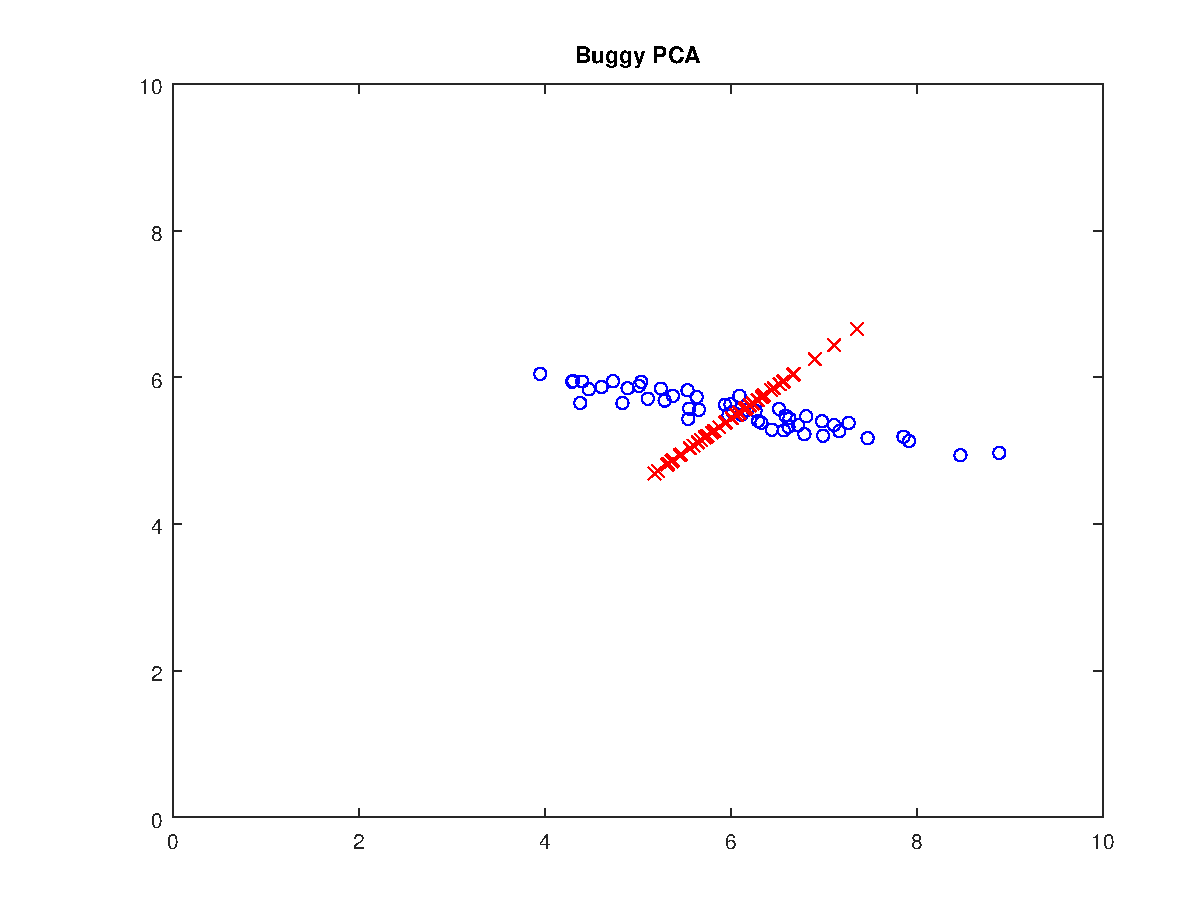
\includegraphics[width=3in]{pcaprog/buggy_pca} \hspace{0.4in}
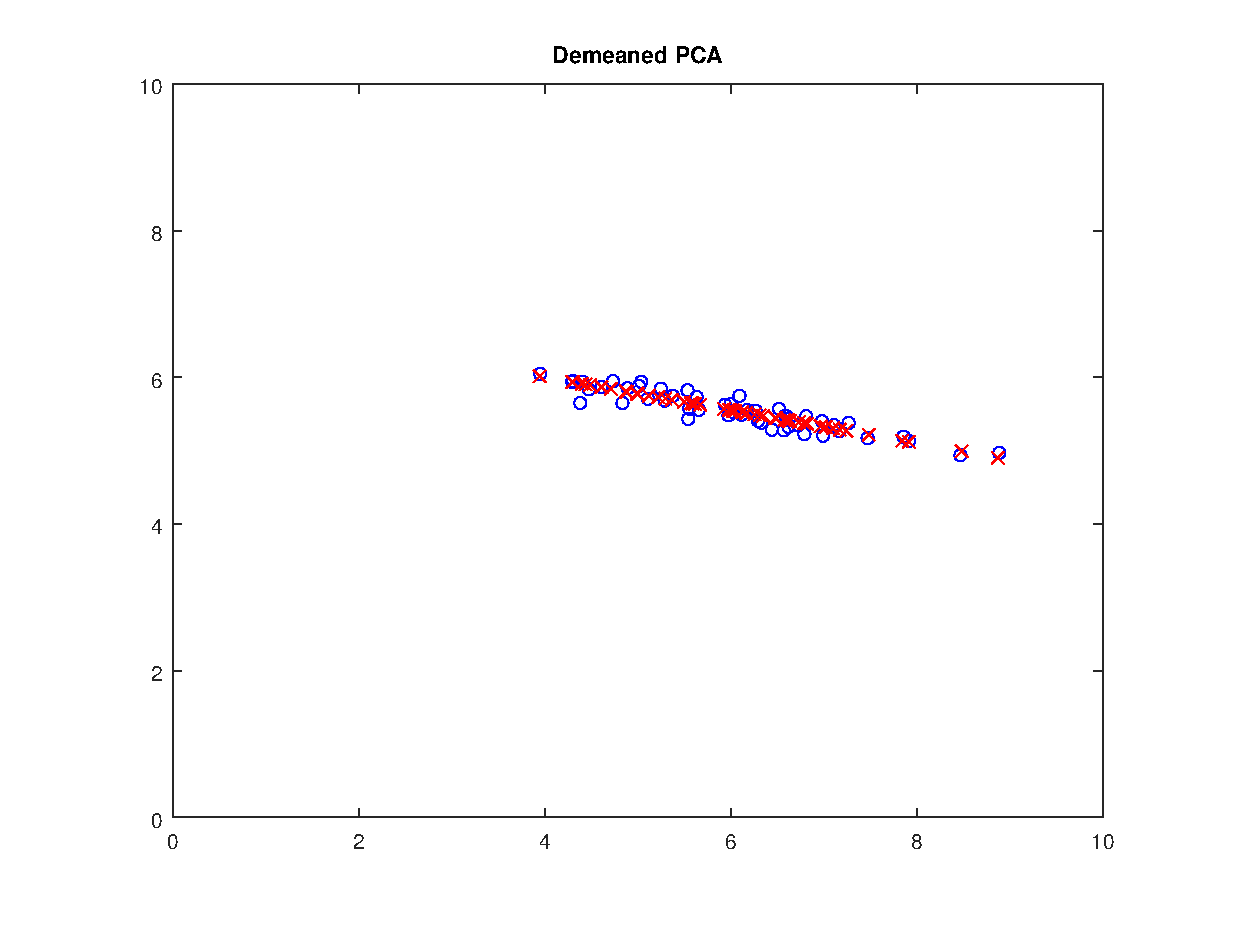
\includegraphics[width=3in]{pcaprog/demeaned_pca} \\
The blue circles are from the original dataset and the red crosses are the reconstructed points.

\vspace{0.2in}

\begin{soln}

    For 2D dataset the Reconstruction Errors are:
    \begin{itemize}
        \item Buggy PCA : 0.886903
        \item Demeaned PCA : 0.010006
        \item Normalized PCA : 0.04947
        \item DRO : 0.010006
        \item DRLV : 0.01212
    \end{itemize}

    \begin{figure}[H]
        \begin{subfigure}{0.5\textwidth}
            \centering
            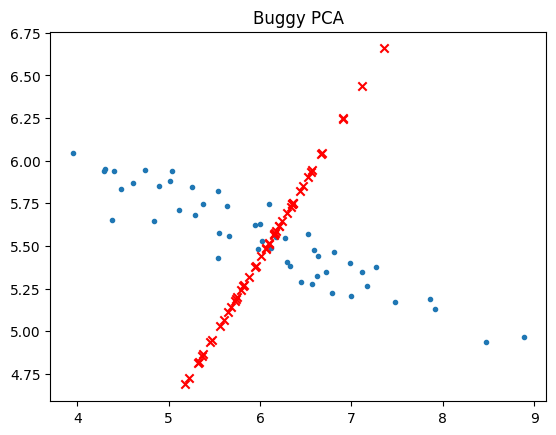
\includegraphics[scale=0.35]{Images/q24/q24_bugpca.png}
        \end{subfigure}%
        \begin{subfigure}{0.5\textwidth}
            \centering
            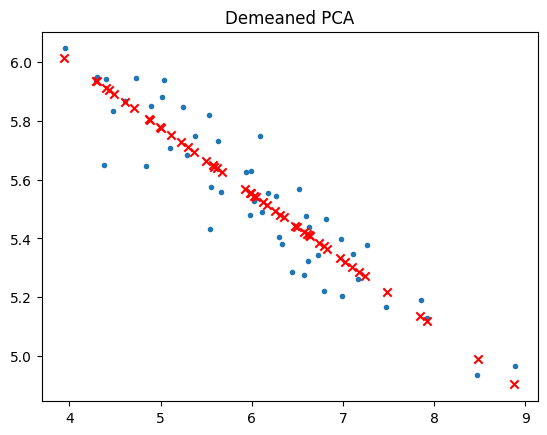
\includegraphics[scale=0.35]{Images/q24/q24_demeanpca.png}
        \end{subfigure}
    \end{figure}
    \begin{figure}[H]
        \begin{subfigure}{0.5\textwidth}
            \centering
            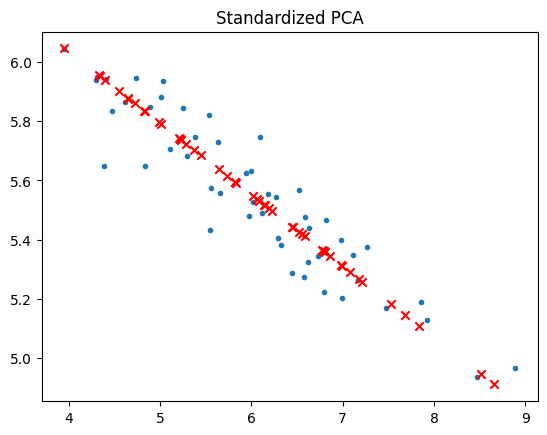
\includegraphics[scale=0.35]{Images/q24/q24_standpca.png}
        \end{subfigure}%
        \begin{subfigure}{0.5\textwidth}
            \centering
            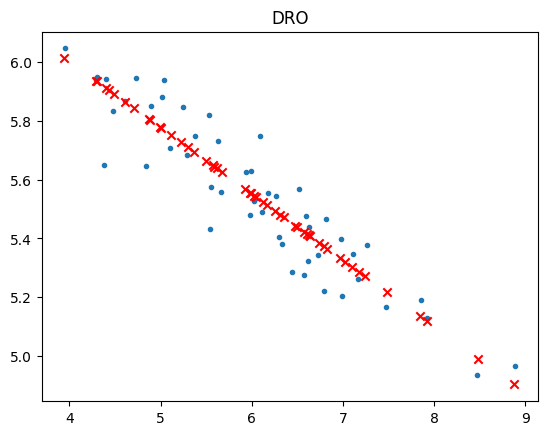
\includegraphics[scale=0.35]{Images/q24/q24_dro.png}
        \end{subfigure}
    \end{figure}
    \begin{figure}[H]
        \centering
        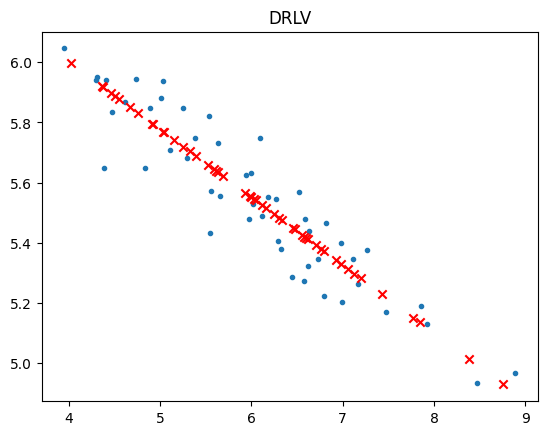
\includegraphics[scale=0.35]{Images/q24/q24_drlv.png}
    \end{figure}

    For 1000D dataset we first estimate the lower dimension using \textbf{cumulative explained variance}. 
    
    \begin{figure}[H]
        \centering
        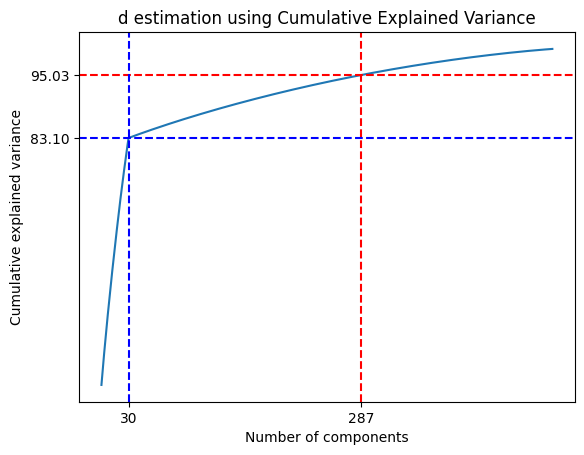
\includegraphics[scale=0.4]{Images/q24/q24_d_est.png}
    \end{figure}

    Error using d=30 dimensions:
    \begin{itemize}
        \item Buggy PCA Loss : 802.731
        \item Demeaned PCA Loss : 273.046
        \item Standardized PCA Loss : 273.629
        \item DRO : 273.046
        \item DRLV : 273.130
    \end{itemize}

    Error using d=300 dimensions:
    \begin{itemize}
        \item Buggy PCA Loss : 43.384
        \item Demeaned PCA Loss : 43.06
        \item Standardized PCA Loss : 44.567
        \item DRO : 43.06
        \item DRLV : Too long to run
    \end{itemize}
\end{soln}

\textbf{Choice of d for 100D}
    
\begin{soln}
    The number of dimensions after which we can explain atleast 95\% of the variance in the dataset is considered a good number of components for PCA. In our case that number turns out of 287. Rounding it upto an even 300 is a good number of components and much less than the original 1000 we had.

    We also observe a knee point at around \textbf{30 components} which is able to explain 83.10\% variance in the data and while its a good estimate with much less number of components its not always be a satisfactory estimate and may result in errors which we see above.\\
\end{soln}


    \textbf{Questions}
    \begin{enumerate}
        \item Look at the results for Buggy PCA. The reconstruction error is bad and the
        reconstructed points don't seem to well represent the original points. Why is
        this? \\
        \textbf{Hint: } Which subspace is Buggy PCA trying to project the points
        onto?
        
        \begin{soln}
            When we perform PCA, the principal components are a subspace of origin-centered vectors. All the principal components pass through the origin as they are just a linear combination of the original components, which also pass through the origin. Hence, we don't center the data before applying PCA; the new components do not consider the shift in data and try to fit the components along the data in the best way possible, resulting in error. \cite{22329}
            \begin{figure}[H]
                \centering
                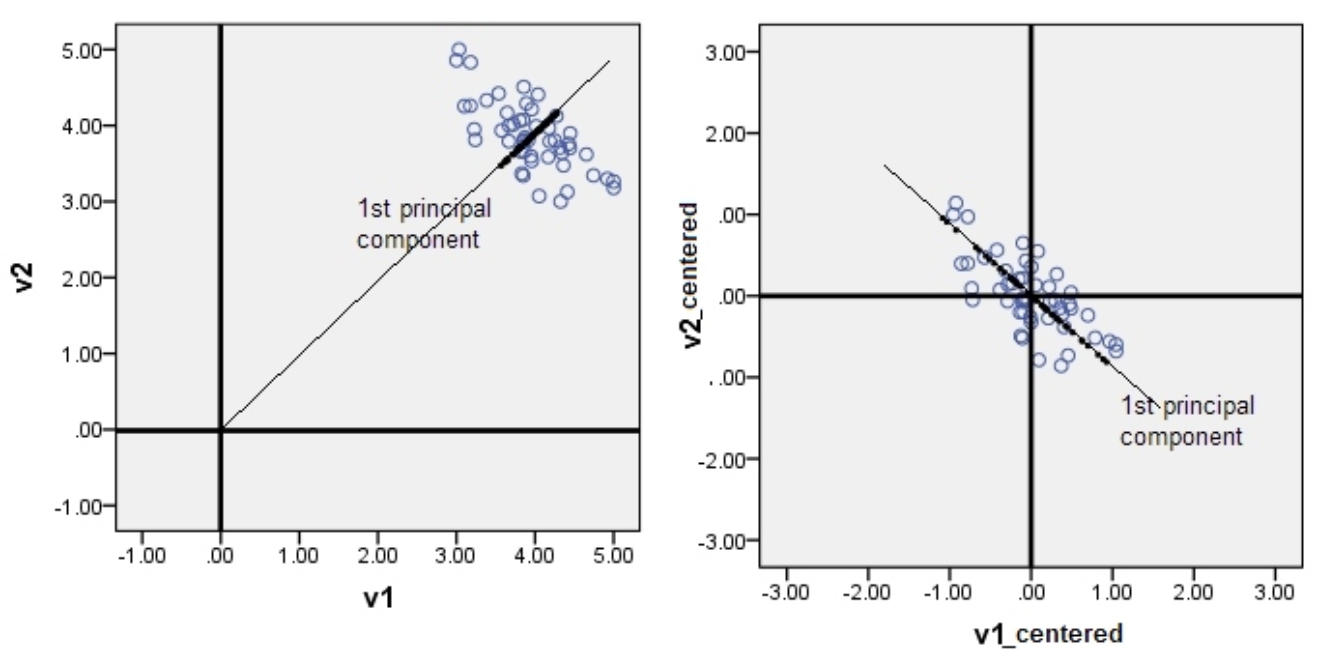
\includegraphics[scale=0.5]{Images/q24/q24_q1_ref.png}
            \end{figure}
        \end{soln}
        \item The error criterion we are using is the average squared error 
        between the original points and the reconstructed points.
        In both examples DRO and demeaned PCA achieves the lowest error among all
        methods. 
        Is this surprising? Why?
        
        \begin{soln}
            We can clearly see that DRO and Demeaned PCA use the same final closed-form solution to arrive at the error. When we see DRO, it tries reducing the Mean squared error(MSE) as its objective function, which is also our error evaluation function and hence has the least error. DRLV tries reducing the log-likelihood, which is not directly related to MSE; Buggy PCA has the issue of demeaning; and Standardized PCA, while being more accurate for general representation, fails here as it also captures inter-dimensional variance and not just the variance in the actual data.
        \end{soln}
    \end{enumerate}



\bibliographystyle{apalike}
\end{document}


